\documentclass{amsart}
\usepackage{amsmath}
\usepackage{amsfonts}
\usepackage{amssymb}
\usepackage{amsthm}
\usepackage{color,hyperref}
\usepackage[table,usenames,dvipsnames]{xcolor}
\usepackage{tikz}
\usetikzlibrary{matrix,arrows,positioning,automata}
\pgfdeclarelayer{background layer}
\pgfsetlayers{background layer,main}

\definecolor{gray9}{gray}{0.9}
\definecolor{gray8}{gray}{0.8}
\definecolor{gray7}{gray}{0.7}
\definecolor{gray6}{gray}{0.6}

\definecolor{darkblue}{rgb}{0.0,0.0,0.3}
\hypersetup{colorlinks,breaklinks,
            linkcolor=darkblue,urlcolor=darkblue,
            anchorcolor=darkblue,citecolor=darkblue}

\usepackage[norelsize,ruled,vlined,linesnumbered]{algorithm2e}

\newcommand{\cT}{{\mathcal T}}
\newcommand{\cS}{{\mathcal S}}
\newcommand{\Sub}{\mathbf{Sub}}
\newcommand{\Set}{\mathbf{Set}}
\newcommand{\Miss}{\mathbf{m}}
\newcommand{\Closure}{\mathbf{Cl}}
\newcommand{\Pos}{\mathbf{Pos}}
\newcommand{\Max}{\mathbf{Max}}
\newcommand{\compl}{\mathsf{c}}

\DeclareMathOperator{\Aut}{Aut}

\newcommand{\todo}[1]{\textcolor{red}{ \small \textsf{[TODO:  #1 ]} \normalsize}}

\theoremstyle{plain}
\newtheorem{theorem}{Theorem}[section]
\newtheorem{lemma}[theorem]{Lemma}
\newtheorem{fact}[theorem]{Fact}
\newtheorem{Proposition}[theorem]{Proposition}
\newtheorem{cor}[theorem]{Corollary}
\theoremstyle{definition}
\newtheorem{definition}[theorem]{Definition}
\newtheorem{example}[theorem]{Example}
\newtheorem{problem}[theorem]{Problem}

\newcommand{\SgpDec}{\textsc{SgpDec}}
\newcommand{\GAP}{\textsc{Gap}}
\newcommand{\Viz}{\textsc{Viz}}
\newcommand{\GraphViz}{\textsc{GraphViz}}



\begin{document}
\title{On Enumerating Transformation Semigroups}
\author{James East$^1$ and Attila Egri-Nagy$^{1}$ and James D. Mitchell$^2$}
\address{$^1$Centre for Research in Mathematics, School of Computing, Engineering and Mathematics, University of Western Sydney (Parramatta Campus), Locked Bag 1797, Penrith, NSW 2751, Australia}
\address{$^2$ Mathematical Institute, University of St Andrews, North Haugh, St Andrews, Fife, KY16 9SS, Scotland}
\email{J.East@uws.edu.au,\ A.Egri-Nagy@uws.edu.au,\ jdm3@st-and.ac.uk}

\maketitle
\begin{abstract}
We describe a multiplication table based calculation method for enumerating all subsemigroups of a semigroup and an algorithm for deciding the isomorphism of semigroups.
We enumerate all transformation semigroups up to degree 4.
In order to make the calculation practically feasible  we had to exploit the ideal structure and the automorphism group of the full transformation semigroup.
\end{abstract}
\tableofcontents
\section{Introduction}
For studying some finite structures  it is often helpful to generate small example objects of that kind by computer programs.
By looking at sample objects we can formulate new hypotheses.
More diverse sample sets make the hypotheses stronger, or easier to falsify them by finding counterexamples.
Therefore, we naturally aim for enumerating all objects of certain size and for increasing the size parameter.

Previous efforts for enumerating semigroups were focused on the abstract case, enumerating by the order, and worked by finding all valid multiplication tables of the given size \cite{For55,tamura1,tamura2,Ple67,KRS76,JW77,SZT94,monoidenum2009}.
Here we enumerate transformation semigroups by degree.
For degree $n$ this is the task of enumerating all valid subtables inside one big multiplication table of the  full transformation semigroups $\cT_n$.

There are several combinatorial and linear representations of semigroups, each them with its own way of multiplying elements, with varying efficiency.
The fastest way to calculate a product is just to look it up in a table, hence we choose the multiplication table as the main way of representing semigroups.
This decision has two consequences. 
First, our algorithms fall into the class of semigroup algorithms that fully enumerate the elements. This of course  restricts us to relatively small semigroups.
Second, our algorithms are completely representaion agnostic.

In Section \ref{sec:multab} we describe methods to work with multiplication tables.
In Section \ref{sec:enum} we describe techniques and algorithms to enumerate subsemigroups of semigroups.
Finally, in Section \ref{sec:fulltranssgp} we apply the developed methods for enumerating transformation semigroups acting on up to 4 points.
\section{Notation}
%Let $(X,S)$ be a transformation semigroup, $n=|S|$.
Let $S$ be finite a semigroup, $n=|S|$.
We fix an order on the semigroup elements $s_1,\ldots, s_n$, so we can easily refer to the elements by their indices. 
Then the  \emph{multiplication table}, or \emph{Cayley-table} of $S$ is a $n\times n$ matrix $M(S)$ or simply $M$ with entries from $\{1,..,n\}$ such that $M_{i,j}=k$ if $s_is_j=s_k$.
$M_A$ denotes the subarray of $M$ spanned by $A\subseteq\{1,\ldots,n\}$.
$R_i$ is the $i$th row and $C_j$ is the $j$th column vector of $M$.
We denote the set of the elements of a vector $v$ by $\Set(v)=\{x\mid x\in v\}$.
Similarly for multiplication tables or subarrays, $\Set(M_A)=\{x\mid x\in M_A\}$.
$\Pos(v,i)$ is the set of positions in vector $v$ containing the value $i$.

$\Sub(S)=\big\{T\mid T\leq S \big\}$ the set of all subsemigroups of $S$, $\Max(S)$ the set of maximal proper subsemigroups of $S$.

If $I$ is an ideal of $S$ then the \emph{Rees factor semigroup} $S/I$ has elements $(S\setminus I)\cup\{0\}$ with multiplication same as in $S$ if the product stays in $S\setminus I$ and zero otherwise.

$\cS_n$ denotes the \emph{symmetric group}, $\cT_n$ the \emph{full transformation semigroup} on $n$ points.
We consider the empty set a semigroup.

\section{Multiplication Table Algorithms}
\label{sec:multab}

\subsection{Closure Algorithms}
A typical question in computational semigroup theory is that given a subset $A$ of a semigroup $S$, what is $\langle A\rangle\leq S$,  the subsemigroup generated by $A$?
What other elements do the elements in $A$ yield when combining them in products?
Since the multiplication table encodes all the products, we can do the calculation on the table. 
Therefore, parallel to the notion of the subsemigroup generated by $A$ we define the \emph{closure} of $A$ as the minimal subarray containing $M_A$.
%and a set of elements  $A\subseteq S$, the  of $T$ by $A$ is $\langle T\cup A \rangle$.
%In particular, when $T=\varnothing$  the closure is $\langle A\rangle$, simply  the subsemigroup the set $A$ generates.
To calculate the closure first we need to determine the missing elements $\Miss(B)=\Set(M_B)\setminus B$, the ones that are referenced in the subarray, but not part of it.
Then, recursively
\begin{align*}
\Closure_1(A)&=A\cup\Miss(A)\\
\Closure_{i+1}(A)&=\Closure_1(\Closure_{i}(A))
\end{align*}
and
$ \Closure(A)=\Closure_j(A), \text{ where $j$ is minimal for }\Closure_j(A)=\Closure_{j+1}(A)$, or equivalently $\Miss(\Closure_j(A))=\varnothing$.

The recursive definition describes an algorithm for calculating the closure, but not an efficient one. Next we discuss some techniques that can be applied to improve the calculation.

\subsubsection{Incremental Method}
We aim to eliminate double checking entries in the table.
If $\Miss(A)$ is already calculated, then all new missing elements in $\Miss(A\cup\{i\})$ should come from the $i$th row and column.
So, for calculating the closure we extend the subarray one-by-one, putting any new missing elements into a list of elements waiting for their inclusion.

\subsubsection{Local Tables}
With additional data structure, the number of checks can be further reduced. 
In the incremental method we ask: Given $A\subseteq S$, what do we need to add when including a new element $i$?
There, the answer is calculated by scanning thorough $R_i$ and $C_i$.

Here we turn around the question.
Do we have to include an element $k$? The answer is given by checking the precalculated positions of $k$. 
Let $V_i=\Set(R_i\cup C_i)$, the values in generated by $i$. Then the  local information table for element $i$ is defined by
$$L_i=\bigcup_{k\in V_i}\left\{(k,\Pos(R_i,k)\cup\Pos(C_i,k))\right\}.$$
For instance if $(k,\{j,h\})\in L_i$ then either $s_is_j=s_k$ or $s_js_i=s_k$ and the same for $s_h$.
Local tables store information local to an element, the content of the corresponding row and column, in a nonredundant way.
When  extending $A\subseteq S$ by $i$, we check $L_i$ for each value $k$ not in $A$ whether its positions contain some elements from $A$. 

This method trades memory and preparation time for speed. Whether it realizes actual speed increase depends on the semigroup $S$ and many implementational details.

\subsubsection{Global Tables}
When $A$ is relatively big in $S$, it makes sense to go through all $k\in S\setminus A$ and ask whether $k\in\Closure(A)$. 
In order to answer this, we need to decide quickly whether there exists $i,j\in A$ such that $s_is_j=s_k$ or $s_js_i=s_k$.
In other words, we need to know the positions of $k$ in $M_s$, encoded by $i,j$ coordinate pairs.
It does not matter whether $s_is_j=s_k$ or $s_js_i=s_k$, so we can talk about ordered pairs $(i,j)$, $i\leq j$ for the coordinates. 
For the purpose of calculating the closure, we can also omit coordinate pairs $i,j$ where $i=k$ of $j=k$. 
Let's denote the set of these pairs by $P_k$.

The set $P_k$ of all coordinate pairs encoding the locations is still redundant in a sense that instead of storing all pairs including $i$, we can simply record $i$ and all second  elements in  pairs where $i$ is the first element.
For instance $(i,j)$ and $(i,h)$ can be stored as $(i,\{h,j\})$, therefore $i$ is only checked once.
Then the  global information table of $k$ is defined by
$$G_k=\bigcup_{(i,j)\in P_k} \left\{ (i,\{j\mid i\leq j\})\right\}.$$

\subsection{Isomorphism and Anti-Isomorphism of Multiplication Tables}
Two semigroups $S$ and $T$ are isomorphic or anti-isomorphic if $M(S)$ can be transformed into $M(T)$ by rearranging its columns and rows and transposing the table.
By computing some global properties of the multiplication tables that are invariant under these rearrangings in some cases we can easily decide non-isomoprhism.
%These are the \emph{table level invariants}.
If all invariants check out, then we can use backtrack to find out whether one of the multiplication tables can be rearranged to get the other one.
An element of $C_2\times S_n$ can witness the isomorphism.
Fortunately we do not have to search through the whole symmetric group, we only need to consider some special permutations that take an element to another one with the same type.
Type is defined by the following invariants.
The search space can be reduced by aligning elements with the same profile (frequency, diagonal frequency, index-period).

\subsubsection{Element Types}

\begin{enumerate}
\item Frequency: the number of occurences of the element in the table.
\item Diagonal frequency: the number of occurences of the element in the diagonal of the table.
\item Index-period: the smallest values $m\geq 1$, $r\geq 1$ such that $a^{m+r}=a^m$.
\item Row and column partition: encoding how many distinct elements are in the right and left principal ideals and what are their frequencies.
\end{enumerate} 

\subsubsection{Table Invariants}

Any property that does not contain information about the ordering of the elements can be used as an invariant.
\begin{enumerate}
\item Distinct frequency values of elements in the table and the number of elements with a given frequency. Useless for groups as their multiplication tables are Latin squares.
\item Column and row partitions types.   Useless for groups since all the principal ideals are the same.
\item The diagonal partition. $|S|=n$ partitioned as a sum of number of occurences of elements in the diagonal. This can even tell some groups apart: $C_4\mapsto 2+2$, $C_2\times C_2\mapsto 4$, but it assings 2+6 to both $D_8$ and $Q_8$.
\item Distinct composite element types: putting together all the element types. In the group case this invariant reduces to the order of elements, but it can distinguish between $D_8$ and $Q_8$. However, this invariant fails to detect the difference between some direct and semidirect products. For instance, $C_8\times C_2$ and $C_8\rtimes C_2$ both have 1 element of order 1, 3 of order 2, 4 of order 4, and 8 of order 8.
\end{enumerate} 



\section{Subsemigroup Enumeration Algorithms}
\label{sec:enum}


\begin{problem}
For a semigroup $S$ find all of its subsemigroups:
$$\Sub(S)=\left\{ X\subseteq S\mid \langle X\rangle=X\right\}.$$
\end{problem}
Thinking in terms of the multiplication table $M$ of $S$, we are looking for subarrays $M_X$ that are also multiplication tables, i.e.\ they do not contain elements not in $X$, $\Set(M_X)=X$.

The obvious brute-force algorithm for constructing $\Sub(S)$ is the enumeration of the powerset $2^S$ and check each subset whether it is closed or not.
However, since we are dealing with algebraic structures, we have many mathematical results to exploit, instead of doing a blind search.

\subsection{Maximal Subsemigroups}
Assuming that we have the maximal subsemigroups calculated, we can parallelize enumerating subsemigroups by enumerating subsemigroups of its maximal subsemigroups and merge the results.
\begin{fact}
$\Sub(S)=\big( \bigcup_{T\in \Max(S)}\Sub(T)\big)\cup \{S\}$
\end{fact}
%\proof
%It follows from the fact that $\Sub(S)$ is an algebraic lattice.
%\qed
\noindent Constructing $\Max(S)$ is described in \cite{MaxSubSemi} and implemented in \cite{Semigroups}.
However, the sets of subsemigroups of the maximal subsemigroups do overlap in general, therefore the same subsemigroup gets enumerated many times and merging is a non-trivial step.
Also, recursively iterating the maximal subsemigroups is a variant of the depth-first search algorithm.  

\subsection{Exploiting Symmetries}
If we know all the symmetries of $S$, the semigroup's automorphism group, then we can accelerate any subsemigroup enumeration algorithm.
Whenever a subsemigroup is found, we can generate its conjugate subsemigroups.
\begin{fact}
$T\in\Sub(S)$ and $g\in \Aut(S)$ then $T^g\in\Sub(S)$.%$g^{-1}Tg\in\Sub(S)$.
\end{fact}
%\proof
%Let $s,t\in T$ and $T'=g^{-1}Tg$.
%$$g^{-1}sgg^{-1}tg=g^{-1}stg.$$
%\qed

If $G$ is a group generated by automorphisms of $S$, then we denote the set of conjugacy class representatives by $\Sub_G(S)$. For $\cT_n$ the automorphism group is $\cS_n$, so we are primarily interested in $\Sub_{\cS_n}(\cT_n)$.

\subsection{Enumerating by Minimal Closures}



The idea is the simplest possible: given a subsemigroup $T\leq S$ we construct all the minimal subsemigroups that contain $T$.
These are obtained by adding one extra generator from $S\setminus T$ (Algorithm \ref{alg:minclosure}).
This algorithm is a depth-first search and its efficiency comes from the fact that the search is cut at subsemigroups already known. 
\begin{algorithm}
\SetKwInOut{Input}{input}\SetKwInOut{Output}{output}
\SetKwData{subs}{subs}
\SetKwFunction{MinClosure}{MinClosure}
\Input{$S$ - the ambient semigroup,\\ $T\leq S$ -  a subsemigroup,\\\subs\ - a set storing subsemigroups already constructed,\\ $s\in S$ - a semigroup element to be added as new generator}
\Output{\subs with all possible extensions of $T$ added}
\SetKwInOut{Name}{\MinClosure($T$,$s$,$S$,\subs)}
\BlankLine
\Name{}
$T'$ $\leftarrow$ $\langle T\cup\{s\}\rangle$\\
    \If{$T'\notin$ \subs}{
      \subs$\leftarrow$ \subs$\cup\{T'\}$\\
      \For{$t\in S\setminus T'$}{
      \MinClosure($T',t,S$,\subs)
    }
  }
\caption{Finding all subsemigroup containing $T$ in $S$. In particular, \textsf{subs} $\leftarrow$ $\varnothing$,  \textsf{Extend}($\varnothing,s,S$,\textsf{subs}) for all  $s\in S$ enumerates all subsemigroups of $S$.}
\label{alg:minclosure}
\end{algorithm}

\subsection{Equivalent Generators}

We define an equivalence relation on $S$ by
$$ s\equiv t \Longleftrightarrow \langle\{s\} \rangle= \langle\{t\} \rangle.$$
For distinct elements this can only happen to nontrivial elements of cyclic groups of prime order.
However, a semigroup can contain many copies of those.
Beyond the obvious copies with fixed points, we have examples that also move the point not in the cycle. For instance, in the singular transformation semigroup of degree 4, $[ 2, 3, 1, 1 ]$ is equivalent to  $[ 3, 1, 2, 2 ]$, both generating $\{ [ 2, 3, 1, 1 ], [ 3, 1, 2, 2 ], [ 1, 2, 3, 3 ]\}$.

In a search algorithm, if $s\equiv t$, then after extending by $s$ we can simply omit extending by $t$.
\subsection{Parallel Enumeration in Ideal Quotients}
In general, an ideal $I$ divides a subsemigroup into two parts: a subsemigroup contained in the ideal and a subset (Fig.\ \ref{fig:torsos}).
The subset also can be made into a subsemigroup by adjoining a zero element, exactly as in a Rees quotient. 
Subsemigroup enumeration can be done in parallel in $I$ and $S/I$  and then  we can combine the results.

\begin{lemma}
Let $I$ be an ideal of $S$, then $$\Sub(S)=\big\{\langle (U\setminus\{0\})\cup L \rangle\mid U\in \Sub(S/I), L\in\Sub(I)\big\}.$$
\end{lemma}
\proof
\qed

\begin{figure}
\begin{center}
\def\S{(0,0) ellipse (1.7cm and 3cm)}
\def\I{(0,-1.7) ellipse (3cm and 2cm)}
\def\T{(-.2,0)ellipse (.8cm and 1.4cm)}
\begin{tikzpicture}
\begin{scope}
\clip\S;
\draw\I;
\draw[very thick]\S;
\end{scope}
\fill [color=gray9] \T;
\draw \T;
\draw (0.3,2.1) node (SI) {$S\setminus I$};
\draw (0.9,2.9) node (S) {$S$};
\draw (0.4,-1.9) node (I) {$I$};
\draw (-0.1,.4) node (T) {$T$};
\end{tikzpicture}
\begin{tikzpicture}
\begin{scope}
\clip\T;
\draw[very thick]\S;
\fill [color=gray9] \T;
\draw\I;
\end{scope}
\draw \T;
\draw (.5,1.2) node (T) {$T$};
\draw (0,-.6) node (L) {$L$};
\draw (-0.3,0.9) node (U) {$U$};
\draw (-2,-2.9) node (invisible) {};%trick for shifting the image
\end{tikzpicture}
\caption{If semigroup $S$ has an ideal $I$, then in general a subsemigroup $T$ is partitioned into two parts, the upper torso $U=T\cap (S\setminus I)$ and the lower torso $L=T\cap I$ by the ideal.}
\label{fig:torsos}
\end{center}
\end{figure}
\section{Enumerating transformation semigroups of degree 2,3 and 4}
\label{sec:fulltranssgp}
In order to enumerate all transformation semigroups on $n$ points we construct all subsemigroups of the full transformation semigroupp $\cT_n$ and use its ideal structure to make the enumeration efficient.
$K_{n,i}$ is the ideal of $\cT_n$ by elements of rank $i$.
$K_{n,n-1}$ is also called the \emph{singular transformation semigroup} of degree $n$.

\subsection{$\cT_2$, The Pen and Paper Case}
Since $\cT_2$ has only four elements and consequently the search space size is only $2^4=16$, it is an easy exercise to find all of its subsemigroups. 
Using one-line notation for transformations, we order the elements lexicographically, 1=[1,1], 2=[1,2], 3=[2,1], 4=[2,2]. Here are the closed subarrays.
\begin{tikzpicture}
[align=center,node distance=2.2cm]
\tikzstyle{plain}=[fill=white,rounded corners=3pt, draw]

\draw node [plain] (1234) {[11],[12],[21],[22]};
\draw node [plain,below left of=1234] (124) {[11],[12],[22]};
\draw node [plain,below of=124] (12) {[11],[12]};
\draw node [plain,left of=12] (14) {[11],[22]};
\draw node [plain,right of=12] (24) {[12],[22]};
\draw node [plain,right of=24] (23) {[12],[21]};

\draw node [plain,below of=12] (1) {[11]};
\draw node [plain,left of=1] (4) {[22]};
\draw node [plain,right of=1] (2) {[12]};
\draw node [plain,below of=1] (empty) {$\varnothing$};

\draw  (1234) -- (124);
\draw (124) -- (12);
\draw (124) -- (24);
\draw (124) -- (14);
\draw  (1234) -- (23);
\path (23) edge (2);
\draw (1) -- (empty);
\draw (2) -- (empty);
\draw (4) -- (empty);
\draw (14) -- (4);
\draw (14) -- (1);
\draw (12) -- (2);
\draw (12) -- (1);
\draw (24) -- (4);
\draw (24) -- (2);
\begin{pgfonlayer}{background layer}
\filldraw [dgr] plot [smooth cycle] coordinates {(1.5,-4.3)(-2.5,-4.2) (-2.3,-3.3) (1.5,-3.4)};
\filldraw [lgr] plot [smooth cycle] coordinates {(-4,-5.2) (2,-5.5) (1,-6.5)(-4.5,-6.6)};
\filldraw [dgr] plot [smooth cycle] coordinates {(-4,-5.5) (-1.2,-5.6) (-1.2,-6.3)(-4,-6.4)};
\end{pgfonlayer}

\end{tikzpicture}
Using these we can draw the subsemigroup lattice (Fig.\ \ref{fig:T2subs}).
\begin{figure}
\begin{tikzpicture}
[align=center,node distance=2.2cm]
\tikzstyle{plain}=[fill=white,rounded corners=3pt, draw]

\draw node [plain] (1234) {[11],[12],[21],[22]};
\draw node [plain,below left of=1234] (124) {[11],[12],[22]};
\draw node [plain,below of=124] (12) {[11],[12]};
\draw node [plain,left of=12] (14) {[11],[22]};
\draw node [plain,right of=12] (24) {[12],[22]};
\draw node [plain,right of=24] (23) {[12],[21]};

\draw node [plain,below of=12] (1) {[11]};
\draw node [plain,left of=1] (4) {[22]};
\draw node [plain,right of=1] (2) {[12]};
\draw node [plain,below of=1] (empty) {$\varnothing$};

\draw  (1234) -- (124);
\draw (124) -- (12);
\draw (124) -- (24);
\draw (124) -- (14);
\draw  (1234) -- (23);
\path (23) edge (2);
\draw (1) -- (empty);
\draw (2) -- (empty);
\draw (4) -- (empty);
\draw (14) -- (4);
\draw (14) -- (1);
\draw (12) -- (2);
\draw (12) -- (1);
\draw (24) -- (4);
\draw (24) -- (2);
\begin{pgfonlayer}{background layer}
\filldraw [dgr] plot [smooth cycle] coordinates {(1.5,-4.3)(-2.5,-4.2) (-2.3,-3.3) (1.5,-3.4)};
\filldraw [lgr] plot [smooth cycle] coordinates {(-4,-5.2) (2,-5.5) (1,-6.5)(-4.5,-6.6)};
\filldraw [dgr] plot [smooth cycle] coordinates {(-4,-5.5) (-1.2,-5.6) (-1.2,-6.3)(-4,-6.4)};
\end{pgfonlayer}

\end{tikzpicture}
\caption{The subsemigroup lattice of $\cT_2$. The horizontal levels correspond to classes of subsemigroups of the same size.  Dark grey blobs indicate nontrivial conjugacy classes, while light grey shows a nontrivial isomorphism class.}
\label{fig:T2subs}
\end{figure}
An obvious classification of $\Sub(\cT_2)$ can be done according to the sizes of the subsemigroups.
Another way of partitioning the elements will also be important for higher degrees. Since we have no problems with calculating $\Sub(\cT_2)$, this division has no significance, but can be visualized easily (Fig.\ \ref{fig:T2subsAlt}).
\begin{figure}
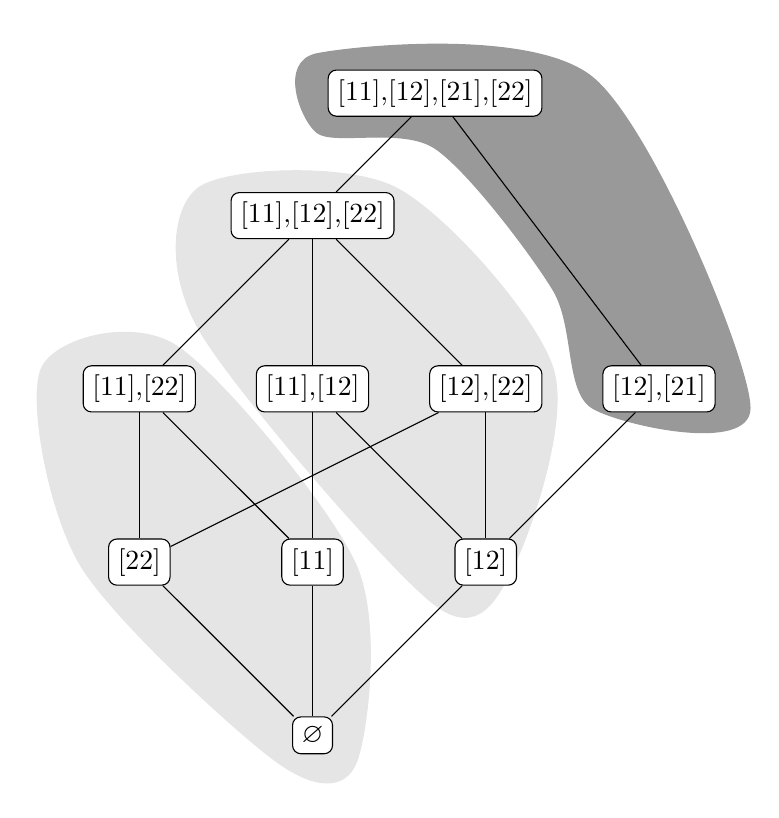
\begin{tikzpicture}
[align=center,node distance=2.2cm]
\tikzstyle{plain}=[fill=white,rounded corners=3pt, draw]

\draw node [plain] (1234) {[11],[12],[21],[22]};
\draw node [plain,below left of=1234] (124) {[11],[12],[22]};
\draw node [plain,below of=124] (12) {[11],[12]};
\draw node [plain,left of=12] (14) {[11],[22]};
\draw node [plain,right of=12] (24) {[12],[22]};
\draw node [plain,right of=24] (23) {[12],[21]};

\draw node [plain,below of=12] (1) {[11]};
\draw node [plain,left of=1] (4) {[22]};
\draw node [plain,right of=1] (2) {[12]};
\draw node [plain,below of=1] (empty) {$\varnothing$};

\draw  (1234) -- (124);
\draw (124) -- (12);
\draw (124) -- (24);
\draw (124) -- (14);
\draw  (1234) -- (23);
\path (23) edge (2);
\draw (1) -- (empty);
\draw (2) -- (empty);
\draw (4) -- (empty);
\draw (14) -- (4);
\draw (14) -- (1);
\draw (12) -- (2);
\draw (12) -- (1);
\draw (24) -- (4);
\draw (24) -- (2);
\begin{pgfonlayer}{background layer}
\filldraw [gray6] plot [smooth cycle] coordinates {(-1.5,-0.5)(-1.5,0.5)(2,0.2)(4,-4)(2,-4)(1.5,-2.5)(0,-0.7)};
\filldraw [gray9] plot [smooth cycle] coordinates {(-0.5,-1.2)(-3,-1.2)(-3,-3)(0,-6.5)(1,-6)(1.5,-3.5)};
\filldraw [gray9] plot [smooth cycle] coordinates {(-3.3,-3.2)(-5,-3.5)(-4.5,-6)(-2,-8.5)(-1,-8.5)(-1,-6)};


\end{pgfonlayer}

\end{tikzpicture}
\caption{The subsemigroup lattice of $\cT_2$, alternative classification. The singular part is indicated by the lowest light gray blob. The other light gray group is an identical copy of the singular part, just the identity adjoined to each subsemigroup. The dark grey part consists of the subsemigroups containing nontrivial permutations. The size of the dark group gets smaller relative to the singular part for higher degrees.}
\label{fig:T2subsAlt}
\end{figure}

\subsection{$\cT_3$, The Brute-force Doable}
Tables \ref{tab:T3freqs} and \ref{tab:T3ngeneratedness}.

\begin{table}
\small
\renewcommand{\tabcolsep}{1pt}
\renewcommand{\arraystretch}{1}
\begin{tabular}{|c|c|c|c|c|c|c|c|c|c|c|c|c|c|c|c|c|c|c|c|c|c|c|c|c|c|c|c|c|}
\hline
Order&0&1&2&3& 4 & 5 & 6 & 7 & 8 & 9 & 10 & 11 & 12 & 13 & 14 & 15 & 16 & 17 & 18 & 19 & 20 & 21 & 22 & 23 & 24 & 25 & 26 & 27\\
\hline
\#conj&1& \cellcolor{gray9}3& \cellcolor{gray9}10& \cellcolor{gray9}19& \cellcolor{gray9}28& \cellcolor{gray9}38&42&38&30&25&14&12&7&3&1&3&2&2& & &  &1&1&1&1& &  &1\\
\hline
\#isom&1& \cellcolor{gray9}1& \cellcolor{gray9}5& \cellcolor{gray9}15& \cellcolor{gray9}24& \cellcolor{gray9}37&42&38&30&25&14&12&7&3&1&3&2&2& & &  &1&1&1&1& &  &1\\
\hline
\end{tabular}
\normalsize
\caption{The frequency distribution of conjugacy and isomorphism classes of $\Sub(\cT_3)$.}
\label{tab:T3freqs}
\end{table}

\begin{table}
\small
\renewcommand{\tabcolsep}{1pt}
\renewcommand{\arraystretch}{1}
\begin{tabular}{|c|c|c|c|c|c|c|c|c|}
\hline
\#generators&0&1&2&3& 4 & 5 & 6 \\
\hline
\#conjugacy classes &1&  7& 46& 101& 85& 36& 7 \\
\hline
\end{tabular}
\normalsize
\caption{$n$-generatedness of conjugacy classes of $\Sub(\cT_3)$. The number of generators in a minimal size minimal generating set and the number of conjugacy classes with that many minimal generators.}
\label{tab:T3ngeneratedness}
\end{table}


\todo{explain frequencies of elements in multiplication table}

\subsection{$\cT_4$, The Parallel Possible }

Calculation steps:

\begin{enumerate}
%\item $\Sub(K_{4,2})$
\item $\Sub(K_{4,3}/K_{4,2})$, these are the upper torsos with a zero adjoined.
\item In parallel, calculate all lower torsos $L$ for all the upper torso $U\in \Sub(K_{4,3}/K_{4,2})$. This gives $\Sub(K_{4,3})$.
\item $P=\left\{\langle G\cup T\rangle\mid G\in\Sub(\cS_4), T\in\Sub(K_{4,3})\right\}$. \todo{JE idea: what we are looking for is the lower torsos fixed by the subgroups of $\cS_4$.}
\item $\Sub(\cT_4)=\Sub(S_4)\cup\Sub(K_{4,3})\cup P$.
\end{enumerate}

\begin{table}
\renewcommand{\tabcolsep}{2pt}
\renewcommand{\arraystretch}{1}
\begin{tabular}{|c|r|r|r||r|r|r||r|r|r|}
\hline
$K_{i,j}$ & \multicolumn{3}{c||}{$j=1$} & \multicolumn{3}{c||}{2} & \multicolumn{3}{c|}{3} \\
\hline
$i=2$ & 4&3&3   & \cellcolor{gray9}  & \cellcolor{gray9}&  \cellcolor{gray9} & \cellcolor{gray9}  &\cellcolor{gray9} &\cellcolor{gray9}\\
\hline
$3$ &  8&4&4  &  600 & 123 & 118  & \cellcolor{gray9}  & \cellcolor{gray9}&\cellcolor{gray9}\\
\hline
$4$ & 16&5&5  &  3788252 & 162332 & 151959  & 1580548624  & 65997018&\\
\hline
$n$ & $2^n$&$n+1$&$n+1$    &    & &    &    & & \\
\hline

\end{tabular}
\caption{Number of subsemigroups of ideals in of full transformation semigroups. The second and third numbers are the number of distinct subsemigroups up to conjugacy and isomorphism.}
\end{table}



\begin{figure}
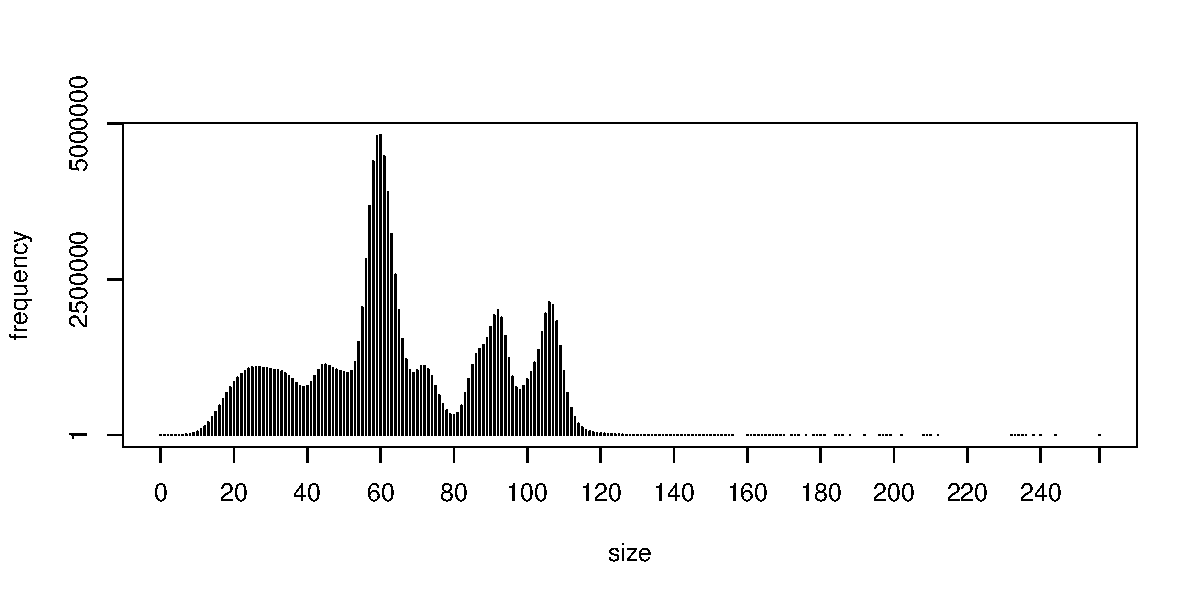
\includegraphics[width=\textwidth]{SubT4distrib}
\caption{The size distribution of $\Sub_{\cS_4}(\cT_4)$. The maximum is at size 60. There are 58 different size values with no subsemigroup (no corresponding dot in the figure).}
\caption{The size distribution of of $\Sub(\cT_4)$. No line/dot is drawn where the value is 0.}
\label{fig:SubT4SizeDistrib}
\end{figure}
The size distribution of $\Sub(\cT_4)$ shows an interesting pattern (Fig.\ \ref{fig:SubT4SizeDistrib}).
For subgroups of a group only the divisors of its order have nonzero frequency values.
For all subsets the maximal binomial coefficient defines the peak value.
For $\Sub(\cT_4)$ the situation is more involved.
The numbers are big and they make the impression of continuous change with several peaks.
To explain the shape of the  distribution a systematic study of the size classes is needed. 
\section{Summary and Conclusion}
We enumerated and classified all transformation semigroups up to degree 4.
It turns out while enumerating abstract semigroups yields mostly 3-nilpotent semigroups, enumerating transformation semigroups gives asymptotically vanishing amount of 3-nilpotents.

The methods developed here, with more concentrated effort and computational power,  may be able to partially enumerate $\Sub(\cT_5)$.
However, a better usage of the results would be to investigate the possibility of a more constructive theory of all transformation semigroups.
For instance, by studying how many different ways $\Sub(\cT_n)$ is embedded into $\Sub(\cT_{n+1})$, we can probably estimate $|\Sub(\cT_{n+1})|$, or even construct some recursive formula.

\begin{table}
\renewcommand{\arraystretch}{1}
\begin{tabular}{|c|r|r|r|}
\hline
 & \#subsemigroups & \#conjugacy classes & \#isomorphism classes \\
\hline
$\cT_0$ & 1  & 1 & 1\\
\hline
$\cT_1$ & 2  & 2 & 2\\
\hline
$\cT_2$ & 10  & 8 & 7\\
\hline
$\cT_3$ & 1299 & 283 & 267\\
\hline
$\cT_4$ & 3161965550 & 132069776 & \\
\hline
\end{tabular}
\caption{Number of subsemigroups of full transformation semigroups.}
\end{table}


\bibliography{subsemi}
\bibliographystyle{plain}

\end{document}